\section{Related Work}
\label{sec:related_work}
\begin{figure*}[ht!]
\begin{subfigure}{0.30\linewidth}
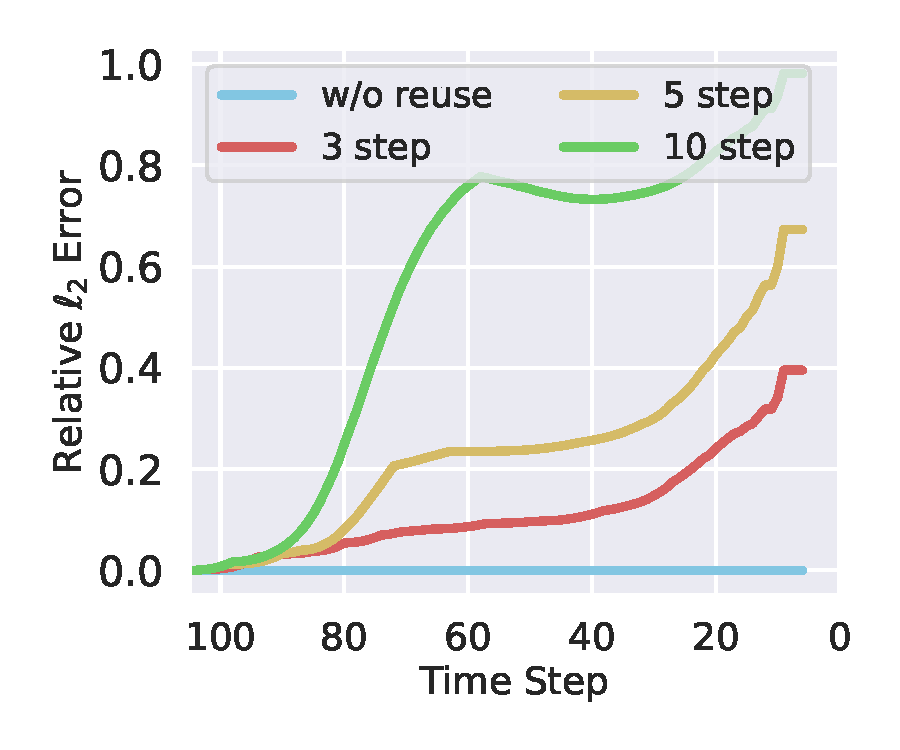
\includegraphics[width=\textwidth]{figures/error_reuse.pdf}
\caption{}
\label{fig:reuse}
\end{subfigure}
\begin{subfigure}{0.69\linewidth}
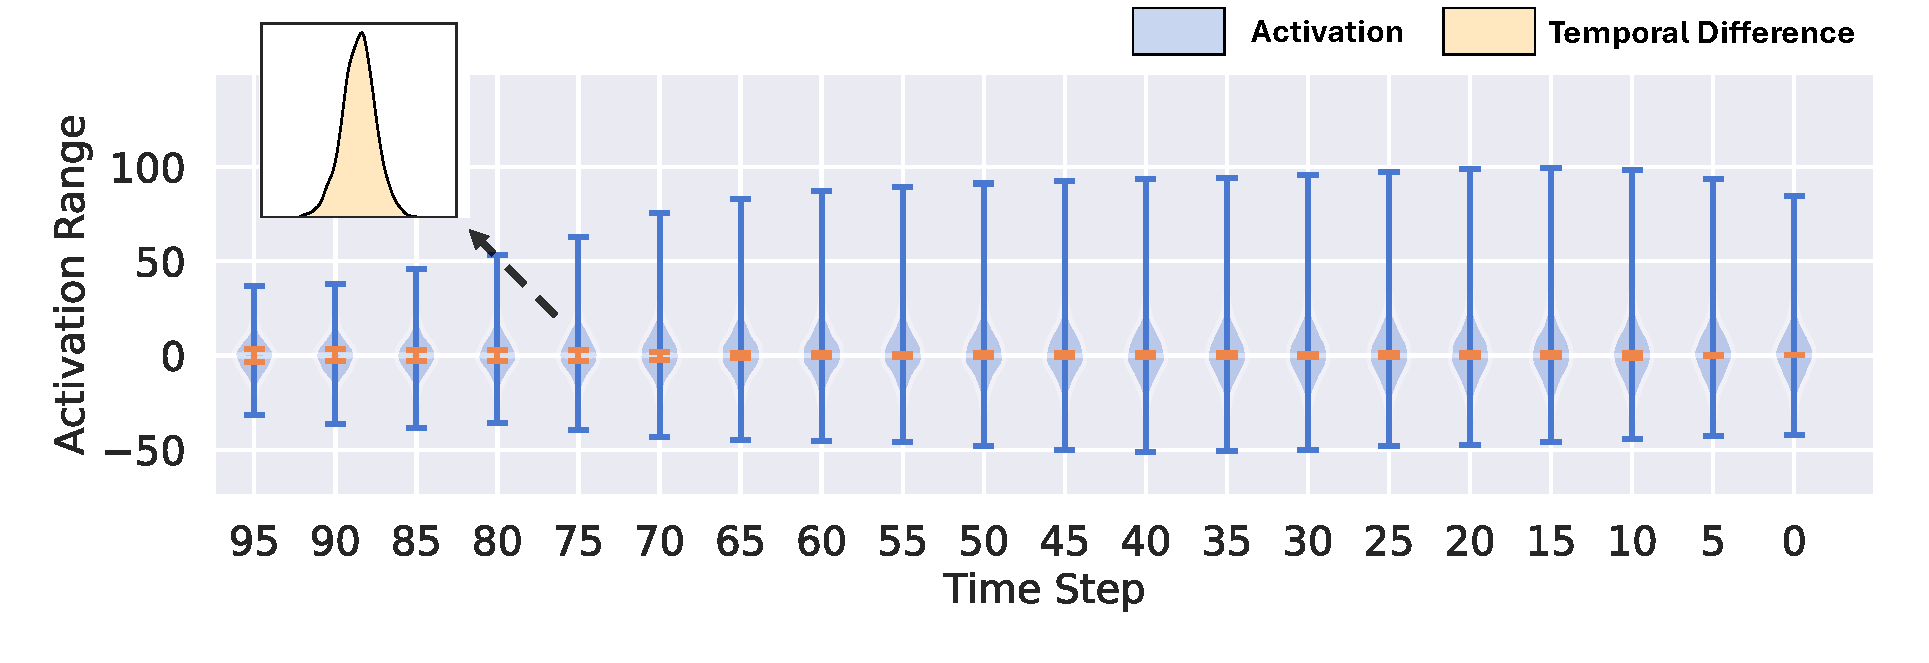
\includegraphics[width=\textwidth]{figures/act_dist.pdf}
\caption{}
\label{fig: activation distribution}
\end{subfigure}
\vspace{-0.1in}
\caption{A preliminary study using DDIM on CIFAR-10 with 100 generation steps. (a) The relative \(\ell_2\) distance between the cached and standard diffusion features in \textit{middle block}, initialized from the same noise. As the reuse frequency increases, error accumulation becomes more significant. (b) The distribution of activations and their temporal differences across different diffusion time steps. The blue violin plots show that activation ranges fluctuate over time and exhibit outliers with long-tailed distributions. In contrast, the orange violin plots demonstrate more consistent ranges and concentrated distributions.
}
\label{fig: prelim}
\end{figure*}

\textbf{Diffusion Models.}
Diffusion models have become a cornerstone of generative modeling, achieving remarkable success across diverse domains such as image synthesis, data distillation, and molecular modeling~\citep{ho2020denoising, hoogeboom2022equivariant, su2024d}. These models operate on an iterative framework that involves adding noise in the forward process and learning to remove it during the reverse process~\citep{dhariwal2021diffusion}. However, the iterative nature of the sampling process makes generation computationally expensive~\citep{song2020score, ho2020denoising}. To address this efficiency bottleneck, a line of research has focused on improving the sampling process by optimizing the variance schedule or employing more advanced ODE solvers~\citep{song2020denoising, nichol2021improved, liu2022pseudo}. For example, Denoising Diffusion Implicit Models (DDIMs) introduce a non-Markovian formulation for the diffusion process, significantly reducing the number of sampling steps required~\citep{song2020denoising}. 

\textbf{Caching Methods.}
Caching methods for accelerating diffusion models aim to reduce redundant computations during the generative process by reusing intermediate results, thereby improving efficiency~\cite{ma2024deepcache,wimbauer2024cache,ma2024learning}. These strategies address the high computational cost by selectively storing intermediate states from the reverse diffusion process for reuse in subsequent steps. For example, DeepCache reuses cached upsampled features every $N$ time steps~\citep{ma2024deepcache}. However, it can accumulate errors in the generation process with the reusing technique. Existing works rely on heuristic approaches to determine $N$, which limits its generalizability. Some methods also attempt to preserve model performance by fine-tuning diffusion models, but this approach can be computationally expensive~\citep{wimbauer2024cache,ma2024learning,chen2024delta}. In contrast to caching methods, our proposed MoDiff introduces a novel and principled framework to leverage the computation redundancy between sampling steps through modulated computing.

\textbf{Post-Training Quantization.}
Quantization aims to reduce inference costs by converting floating-point numbers into low-bit integers~\citep{nagel2021white, yang2019quantization} using scaling factors. Post-training quantization (PTQ) has emerged as a powerful approach due to its training-free nature, making it suitable for pre-trained models~\citep{li2021brecq}. Several studies have explored the application of PTQ techniques to diffusion models~\citep{li2023q, wang2024towards, huang2024tfmq, shang2023post, he2023ptqd, zhao2024vidit}. For example, Q-Diffusion introduces a time-step-aware calibration data sampling mechanism tailored for diffusion models, achieving strong performance with 8-bit activations. However, a common issue is that existing methods struggle to quantize activations to low bitwidths due to the presence of outlier values with large dynamic ranges~\citep{xiao2023smoothquant, feng2024mpq}. {One related method is PTQD~\citep{he2023ptqd}, which post processes quantized models to reduce the quantization error. We pose the detailed comparison to PTQD in Appendix~\ref{appsec:ptqd}.}

Another line of research focuses on quantization-aware training (QAT), which integrates the quantization process into the training phase, enabling model parameters to adapt to quantization~\citep{nagel2022overcoming}. These methods effectively address the challenges of low-bit quantization in diffusion models~\citep{feng2024mpq, he2023efficientdm}. However, QAT approaches require costly retraining of diffusion models, which is \textbf{orthogonal to but not the focus of this work}. In contrast, the proposed MoDiff framework can be seamlessly integrated to state-of-the-art PTQ methods to reduce activation bit-widths without additional training.



